\documentclass[12pt,a4paper]{article}

\usepackage{alltt}
\usepackage[utf8]{inputenc}
\usepackage[english]{babel}
\usepackage{amsmath}
\usepackage{amsfonts}
\usepackage{amssymb}
\usepackage{indentfirst}
\usepackage{setspace}
\usepackage[pdftex]{graphicx}
\usepackage{caption}
\usepackage{subcaption}
\usepackage{textcomp}
\usepackage{array}
\usepackage{listings}
\usepackage{color}
\usepackage{tikz} % для создания иллюстраций
\usepackage{hyperref}

\newcommand{\infers}{\,\to\,}
\newcommand{\tinfers}{\;\Rightarrow\;}

%\voffset = -118pt
%\textheight = 820pt
%\hoffset = -100pt
%\textwidth = 550pt
\newcommand{\htext}{0.46\textwidth}
\newcommand{\hstext}{0.45\textwidth}

\newcommand{\mat}[1]{\vec{#1}}
\newcommand{\framed}[1]{\tikz[baseline=(char.base)]{\node[shape=rectangle,draw,inner sep=4pt] (char) {#1};}}

%opening
\title{}
\author{}

\begin{document}


% TEAM.
\parbox{0.333\textwidth}{
	Maksim Velikanov \\[0mm]
}
% In der Mitte der Name der Veranstaltung.
\parbox{0.333\textwidth}{\vspace*{1mm}\begin{center}\large\bf%
		HPC with C++\\[0mm]
		SS 24\\[0mm]
\end{center}}
\parbox{0.333\textwidth}{
	\begin{flushright}
		Project report\\[0mm]
		17.02.2025\\[0mm]
	\end{flushright}
}
\par\vspace{-5mm}
\definecolor{freiburg-gray}{rgb}{0.68,0.68,0.68}
\vspace*{2mm}
\raisebox{1.19cm}{%
	\textcolor{freiburg-gray}{\rule{\textwidth}{1.1mm}}}

\bigskip




\section{Introduction}

In this project I implemented a Molecular Dynamics simulation in C++ consisting of individual atoms, based on the physics equations for interaction between atoms. The implemented program contains several experiments: running simulation on generated cubic lattice or using a precomputed icosahedron cluster; controlling the temperature of the simulation with a thermostat to prevent vaporization; monitoring the potential and kinetic energies; saving the atom positions to a file and visualization; heating the cluster and measuring the melting point and latent heat; running parallel simulation with OpenMPI; stretching a golden whisker and measuring stress.

The theoretical base is present in \hyperref[methods]{methods} section, the details of implementation and results in \hyperref[experiments]{experiments}, and \hyperref[conclusion]{conclusion} at the end.

\section{Methods}
\label{methods}

The key methods for modeling a physical system of atoms are following:

\begin{enumerate}
	\item Update atom position and velocity, given constant force for a small time step --- {\bf Velocity-Verlet integrator}
	\item Estimate force between particles from the potential energy --- {\bf Lennard-Jones potential}
	\item Stabilization of the system by connecting it to a constant-temperature heat bath --- {\bf Berendsen Thermostat}
	\item Physically accurate N-body potential for modeling metals --- {\bf Embedded Atom Method potential}
	\item {\bf Domain decomposition} and parallel execution with OpenMPI
	\item Application of an external force --- {\bf Stress estimation}
\end{enumerate}

\newpage
\subsection*{Velocity-Verlet integrator}

The atom movement is approximated by assuming constant force and making small time steps. The method was rediscovered by Loup Verlet \cite{verlet} for Molecular Dynamics simulation.

Vector form of Newton's law gives:
\[ \dot{\mat{v}}_i(t) = \cfrac{\mat{f}_i(t)}{m_i} \]

Definition of velocity:
\[ \dot{\mat{r}}_i(t) = \mat{v}_i(t) \]

From these two formulas we get the approximation equations using Taylor formula.
Integration, predictor step:
\[
v_i(t + \Delta t/2) = v_i(t) + \cfrac{1}{2m_i} f_i(t) \Delta t
\]
\[ r_i(t+\Delta t) = r_i(t) + v_i(t+ \Delta t/2) \Delta t \]

After this step we must recompute the forces for new positions of atoms. Corrector step:
\[ v_i(t+\Delta t) = v_i(t+\Delta t/2) + \cfrac{1}{2m_i}f_i(t+\Delta t) \Delta t \]

\subsection*{Lennard Jones potential}

Here we derive a formula to compute the force from potential energy. By definition of pair potential:
\[
E_{pot} = \sum_{i<j} V(r_{ij})
\]

Lennard-Jones potential \cite{lennard-jones} is sum of Pauli Repulsion (repulsive force) and London Dispersion (attractive force). These interactions act even on uncharged atoms.

\[
V_{ij}(r) = 4\epsilon \left( \Bigl(\cfrac{\sigma}{r}\Bigr)^{12} - \Bigl(\cfrac{\sigma}{r}\Bigr)^{6} \right)
\]

By definition of energy, force is the derivative of energy by position.
\[
\mat{f}_k = \left( \begin{aligned}
	& - \partial E / \partial x_k \\
	& - \partial E / \partial y_k \\
	& - \partial E / \partial z_k \\
\end{aligned} \right) = \sum_i \cfrac{\partial V}{\partial r_{ik}} {\hat r_{ik}} \text{\ (unit vector)}
\]

Let's compute derivative of the potential for one of the dimensions.
\[
\cfrac{\partial V_{ij}}{\partial x_k} = \text{(chain rule by vector length)} \cfrac{\partial V_{ij}}{\partial r_{ij}} \cfrac{\partial r_{ij}}{\partial x_k}
\]

\[ \cfrac{\partial r_{ij}}{\partial x_k} = \cfrac{\partial \sqrt{(x_j-x_i)^2 + (y_j-y_i)^2 + (z_j-z_i)^2  }}{\partial x_k} = (*) \]
Remember: \( (\sqrt{u})' = \cfrac{1}{2\sqrt{u}} u' \)

\[
(*) = \cfrac{1}{2r_{ij}} \cfrac{(x_j-x_i)^2+\ldots}{\partial x_k} = \cfrac{1}{r_{ij}} \ (x_j-x_i) \ \Bigl(\cfrac{\partial x_j}{\partial x_k} - \cfrac{\partial x_i}{\partial x_k}\Bigr)
\]
Here is a pair of atoms $i$ and $j$. We want the force for atom $k$. If \(k\neq i\) and \(k\neq j\), the expression is 0.

\[
\cfrac{\partial r_{ij}}{\partial \mat{r_k}} = \left( \begin{aligned}
	& (x_j - x_i) (\delta_{jk} - \delta_{ik}) / r_{ij} \\
	& (y_j - y_i) (\delta_{ik} - \delta_{jk}) / r_{ij} \\
	& (z_j - z_i) (\delta_{ik} - \delta_{jk}) / r_{ij} \\
\end{aligned} \right) = (**)
\]

\[
k=j \infers (x_k-x_i)(1-0)/r_{ik},\ (**) = {\hat r_{ik}}
\]
\[
k=i \infers (x_j-x_k)(0-1)/r_{kj},\ (**) = {\hat r_{jk}}
\]

When we take the derivative of energy, only the pairs, where one of the atoms is \(k\), are left. The derivative is exactly the same for \(V_{ij}\) and \(V_{ji}\).

{\centering\framed{ \( \mat{f}_k = - \sum_i \cfrac{\partial V}{\partial r} {\hat r_{ik}} \) }\\}

Last piece in the puzzle is derivative of potential by distance.

\[
\cfrac{\partial V}{\partial r} = 4\epsilon (\sigma^{12} (-12) r^{-13} - 6 \  \sigma^6 \ r^{-7})
\]

\subsection*{Berendsen thermostat}

As the molecular dynamics system evolves, potential energy decreases and kinetic energy increases. Kinetic energy is temperature multiplied by a constant: $E_k = \frac{3}{2} NK_b T$, so the temperature can get too high and system will explode. Therefore we connect the system to a heat bath of constant temperature, which stabilizes the simulation. The Berendsen thermostat \cite{berendsen} decreases the temperature by scaling the velocities of atoms by a factor:

\[ v' = \lambda v \]

\[ \lambda = \sqrt{1 + \left(\cfrac{T_0}{T}-1 \right) \cfrac{\Delta t}{\tau} }  \]
\[ E_k = \cfrac{1}{2} \sum_i m_i v_i^2 = \cfrac{3}{2} N K_b T \infers T = \cfrac{2}{3} \cfrac{E_k}{K_b N} \]

\(T_0\) is target temperature, \(\Delta t \) is simulation timestep, \( \tau \) is relaxation time of the thermostat and should be much larger than the time step.

\subsection*{Embedded Atom Method potential}

The EAM models attraction with the local electron density, and repulsion with a pairwise term (developed by Ducastelle \cite{ducastelle1970modules}, Gupta \cite{gupta} and Cleri and Rosato \cite{CleriRosato}). This potential has parameters that must be estimated for each type of atom experimentally, in this report we use gold (Au).

Force is the derivative of energy by position:
\[
\mat{f}_k = -\cfrac{\partial E_{pot}}{\partial \mat{r}_k}
\]

\[
\mat{f}_k = \sum_i ( \partial F(\rho_k) / \partial \rho_k + \partial F(\rho_i) / \partial \rho_i )  \cfrac{\partial f}{\partial r_{ik}} \hat{r}_{ik} +
\sum_i \cfrac{\partial V}{\partial r_{ik}} \hat{r}_{ik},
\]

where $\mat{f}_k$ is force on atom $k$, $r_k$ is position of atom $k$, $F(\rho)$ is an embedding functional dependent on electron density, $V$ is pairwise repulsion.

\subsection*{EAM potential, time and mass units}

We create a new convenient unit system for the simulation. First, fix the length to Angstrem (approximately distance between atoms) and energy to electron-volts (energy of a covalent bond):

\begin{itemize}
	\item length: Å, 1 angstrem = 0,1 nm. 1 meter = $10^{10}$ Å
	\item energy: eV, electron-volts (elementary electrical charges) = qU Joules = $1,602 \cdot 10^{-19}$ Volts. 1 Joule = $1/U$ eV
	\item velocity: $[l]/[t]$
	\item acceleration: $[l]/[t]^2$
	\item $f=ma$:       $[m][l]/[t]^2$
	\item $[E]=[A]=[fS]$:    $[m][l]^2/[t]^2$
	\item $f$: $[E]/[l]$
\end{itemize}

Boltzmann constant in new unit system: \[ K_b = 1,38 \cdot 10^{-23} \frac{J}{K} = \frac{1,38}{1,602} \cdot 10^{-23} \cdot 10^{+19} \text{eV/K} = 0,8614 \cdot 10^{-4} = \underline{8,614 \cdot 10^{-5} \text{eV/K}} \]

We fix \underline{[t] = 1 fs}. From this derive the unit of mass $[m]$: 

\begin{gather*}
	[E] = [m][l]^2/[t]^2\\
	[m] = [E][t]^2/[l]^2\\
	[m] = \text{eV} \cdot \text{fs}^2 / \text{Å}^2 =\\
	1,602 \cdot 10^{-19} J \cdot 10^{-30} s \cdot 10^{+20} m = 1,6 \cdot 10^{-29} \text{kg}
\end{gather*}

We can convert this to g/mol:
\begin{center}
	1mol $= 6.02 \cdot 10^{23}$\\
	1 g/mol = $\cfrac{10^{-3}}{6 \cdot 10^{23}}$ kg\\
	1 kg = $6 \cdot 10^{26}$ g/mol\\
	$[m] = 1,6 \cdot 10^{-29} \cdot 6 \cdot 10^{+26} \text{g/mol} = 9,6 \cdot 10^{-3} =$ \underline{0,009649 g/mol}\\
	1 g/mol = $103,63\ [m]$
\end{center}

In the new units 1 gold atom weighs $196,96 \cdot 103,63$ units of mass.

\subsection*{Lennard Jones potential, time and mass units}

To define a unit system, we need to fix three units. For Lennard Jones we set length to Angstrem, energy to electron-volts, and mass to one golden atom (in EAM we instead set the time unit).

\begin{itemize}
	\item length: Å, 1 Angstrem = $10^{-10}$ m
	\item energy: 1 eV, electron-volts = $1,602 \cdot 10^{-19}$ Joules
	\item $[E] = [m][l]^2/[t]^2$
	\item mass of 1 gold atom $[m] = 197 / 6 \cdot 10^{-26}$ kg
\end{itemize}

From this I derive the time unit:

\begin{center}
	$[t]^2 = [m][l]^2/[E] =$\\
	$[m] \cdot \ \text{Å}^2 / \text{eV}$ =\\
	$197 / 6 \cdot 10^{-26}$ kg $\ \cdot \ 10^{-20}$ meter $\ / \ (1.602 \cdot 10^{-19})$ Joules =\\
	$\cfrac{197}{6 \cdot 1.602} 10^{-46 + 19} s^2 = 20 \cdot 10^{-27} s^2$\\
	$[t] = \sqrt{20 \cdot 10^{-27}} s = 1.42 \cdot 10^{-13} s =$ \underline{142 fs}
\end{center}

\subsection*{Domain decomposition}

We fix the region of simulation and divide it into a regular grid. Size of the region is $[0, L_x] \times [0, L_y] \times [0, L_z]$, for each dimension we divide it into $N_x, N_y, N_z$ subdomains. The computation is parallelized by spawning a process for each subdomain. Each process holds all atoms in its subdomain and the atoms near the border of subdomain (ghost atoms) not further than cutoff radius multiplied by 2 for EAM potential.

The processes have to communicate the atom movement and ghost atoms with the neighboring subdomains. Each subdomain has $9+8+9=26$ neighbors in 3D, communicating between each pair would significantly decrease performance. To avoid pair-wise communication between them, we execute send-receive (Fig.~\ref{fig:domain-communication}) in these directions only:

\begin{enumerate}
	\item in $x+$ direction
	\item in $x-$ direction
	\item in $y+$ direction
	\item in $y-$ direction
	\item in $z+$ direction
	\item in $z-$ direction
\end{enumerate}

\begin{figure*}[h!]
	\centering
	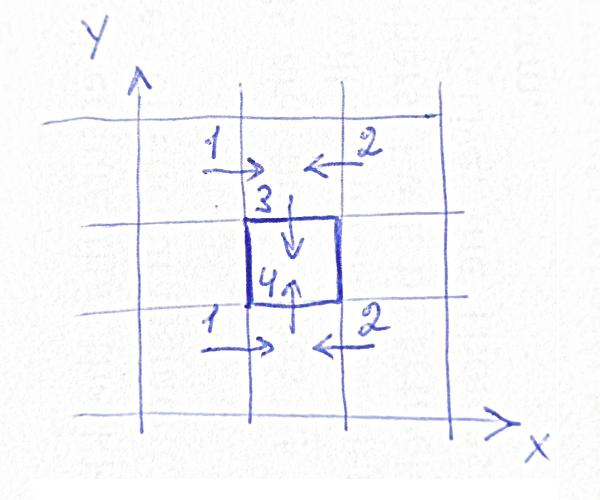
\includegraphics[width=.5\linewidth]{img/milestone08-domain-communication.jpg}
	\caption{Each process gets neighbor information without direct communication between all pairs of processes.}
	\label{fig:domain-communication}
\end{figure*}

This way it takes 6 steps instead of 26 for each process to get all information from its neighbors.

\subsection*{Stress estimation}

For the experiment with stretching a golden whisker we need to compute the reaction to strain --- the stress tensor. It requires to compute a sum over all forces acting on the atoms in the subdomain. Because ghost atoms also act on the atoms inside the subdomain, we must include the force produced by them into the sum, but we must exclude the forces that act on the ghost atoms themselves because they are not part of subdomain.

The stress tensor components correspond to stress in different dimensions. In simulation, we stretch the whisker only in the Z axis, so only $\sigma_{zz}$ is useful. Proving this assumption, all other components of the matrix were close to 0 in the experiment. Stress can be computed separately for each atom and then summed.

\[
\sigma =
\begin{pmatrix}
	\sigma_{xx} &\sigma_{xy} &\sigma_{xz}\\
	\sigma_{yx} &\sigma_{yy} &\sigma_{yz}\\
	\sigma_{zx} &\sigma_{zy} &\sigma_{zz}\\
\end{pmatrix}
\]

\[
\sigma = \cfrac{1}{V} \sum_{i<j} \mat{r}_{ij} \times \mat{f}^T_{ij} = \cfrac{1}{V} \sum_i^{N} \sum_{j=i}^{N+N_G} \mat{r}_{ij} \times \mat{f}^T_{ij},
\]

where $V$ is body volume, $\mat{r}_{ij}$ is position, $\mat{f}_{ij}$ is force, $N_G$ is the number of ghost atoms.

% {\bf Outer product operation}
% \[ C = \mat{a} \times \mat{b}^T, \]
% where $\mat{a}$ has shape $3 \times 1$, $\mat{b}^T$ has shape $1 \times 3$, $C$ has shape $3 \times 3$.

\clearpage

\section{Experiments}
\label{experiments}

Warning! Copying .xyz files in Meson didn't work for me, so I had to copy them to build directory by hand.
	
Code is structured in folders:
\begin{itemize}
	\item milestones --- CPP sources for simulation executables
	\item plot --- Python notebooks for plotting. Requires precomputed simultion results
	\item report --- the sources for the report you are reading now
	\item src --- common CPP files
	\item tests --- CPP tests using Google test framework
\end{itemize}

\subsection*{Velocity-Verlet test}

{\bf First test: constant acceleration.} For $m=1.0$, acceleration is equal to force. The movement distance under constant acceleration is well known: \[ S = v_0 t + \cfrac{at^2}{2} \]

Let's test two cases:\\
first atom with position $\mat{r_1}(1, 0, 0)$ and acceleration $\mat{a_1}(1, 0, 0)$,\\
second atom with position $\mat{r_2}(0, 1, 0)$ and acceleration $\mat{a_2}(0, -0.5, 0)$.\\
Start velocity is 0 for simplicity. The positions at $t = 10$ should be

\[ \mat{r_1}(x, t=10) = 1 + 0 + \cfrac{1 \cdot 100}{2} = 51 \]
\[ \mat{r_2}(y, t=10) = 1 + 0 - \cfrac{0.5 \cdot 100}{2} = -24 \]

The Verlet timestep in this test can be chosen as large as possible -- the computed result always matches the analytical one.

{\bf Second test: linear acceleration.} Let acceleration be a function of time:

\[ a(t) = 1 - t,\; t \in [0, 1] \]

Acceleration is derivative of velocity, so:

\[ a = \cfrac{dv}{dt} \]

For a constant acceleration we use the well known formula to find velocity: \[ a = \frac{v_{end}-v_{start}}{t} \]

But for variable acceleration:

\[ v(t) = \int_0^t a(t) dt + v_0 \]
\[ S(t) = \int_0^t v(t) dt \]
\[ S(t) = \int_0^t \left( \int_0^t a(t) dt + v_0 \right) dt\]

Now compute S using the acceleration expression, with start velocity 0 for simplicity:

\[ v(t) = \int_0^t (1-t) dt = t - t^2 / 2\]
\[ S(t) = \int_0^t (t - t^2/2) dt = t^2/2 - t^3/6 \]

We obtained the analytical solution. Now let's test it on one atom with position $\mat{r}(1, 0, 0)$. At $t=0.5$ the position should be:

\[ \mat{r}(x, t=0.5) = 1 + 0.5^2/2 - 0.5^3/6 = 1 + 5/(8 \cdot 6)\]

In this test the timestep must be small enough to capture the nonlinear changes in the velocity. I achieved approximate equality with $\Delta t = 0.00001$.

{\bf Implementation}
\begin{lstlisting}[breaklines]
src/atoms.h,
src/verlet.cpp,
src/verlet.h,
tests/test_verlet.cpp
\end{lstlisting}

\clearpage

\subsection*{First simulation with Lennard-Jones potential}

The goal of this experiment is to monitor the total energy of the system, running the simulation with different time steps. The Lennard-Jones potential was used to compute forces between atoms. We don't specify the real physical units because we'll be using the Embedded Atom Potential for realistic modelling.

The drift of total energy from initial value was plotted for different time steps in Fig.~\ref{fig:first_simulation}. Timesteps above $0.05 \sqrt{m\sigma^2 / \epsilon}$ caused explosion of the system.

{\bf Implementation}
\begin{lstlisting}[breaklines]
src/lj_direct_summation.cpp, 
src/lj_direct_summation.h,
tests/test_lj_direct_summation.cpp,
src/xyz.cpp,
src/xyz.h,
tests/test_verlet.cpp,
milestones/04/main.cpp
\end{lstlisting}


{\bf Plot} --- \verb|plot/energy_lineplot.ipynb|

\begin{figure*}[htb]
	\centering
	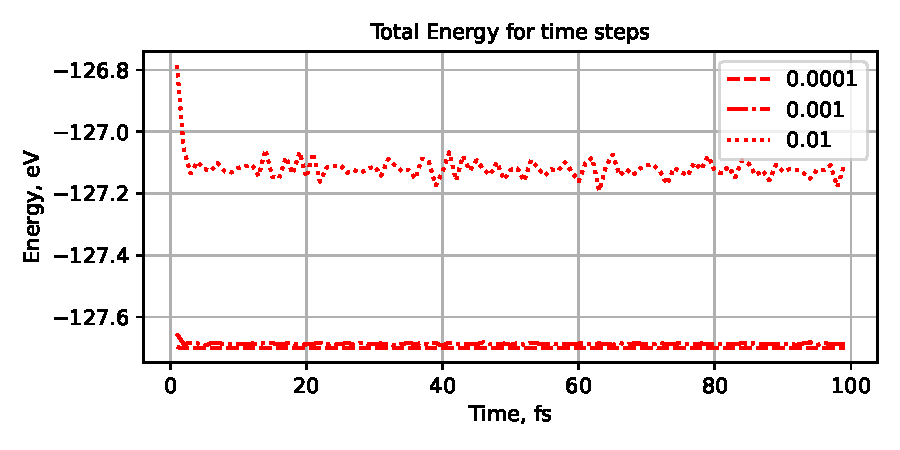
\includegraphics[width=.7\linewidth]{img/milestone04-total.pdf}
	\caption{With smaller time step the energy drift is smaller.\\
		I plot the total energy minus its initial value.\\
		Time is in Lennard Jones time units.\\
		Timesteps in the legend must be multiplied by $\sqrt{m\sigma^2 / \epsilon}$ to get Lennard Jones time units.\\
		Initial atom configuration from file {\bf lj54.xyz}.\\
		Lennard Jones parameters are: $m=1$ LJ units of mass, $\sigma$ = 1Å, $\epsilon$=1 eV.\\
		Total simulation time \( 100 \sqrt{m\sigma^2 / \epsilon} \), simulation state save interval \( 1 \sqrt{m\sigma^2 / \epsilon} \).}
	\label{fig:first_simulation}
\end{figure*}

\clearpage


\subsection*{Berendsen thermostat}

\begin{figure*}[h!]
	\centering
	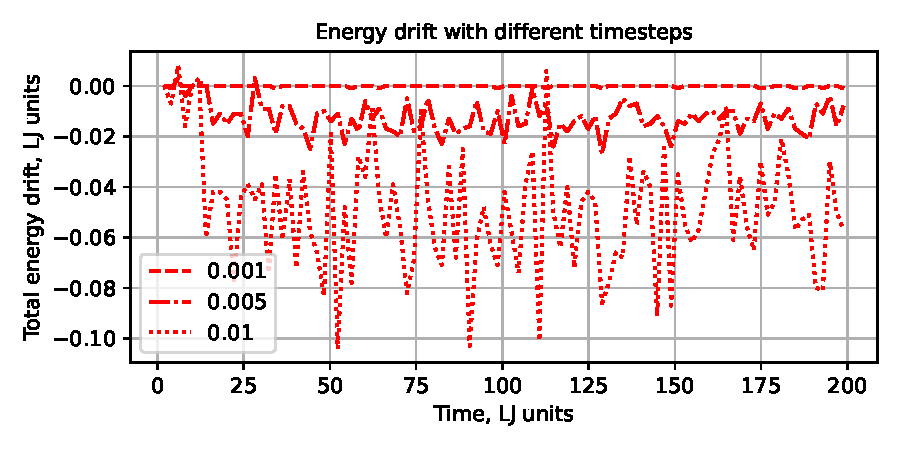
\includegraphics[width=.7\linewidth]{img/milestone05-total.pdf}
	\caption{Choosing the optimal time step for the cube of atoms, which is 0.001 $\sqrt{m\sigma^2 / \epsilon}$ in this case.\\
		I plot the total energy minus its initial value.\\
		Time is in Lennard Jones potential units.\\
		Timesteps in the legend must be multiplied by $\sqrt{m\sigma^2 / \epsilon}$ to get Lennard Jones time units.\\
		Initial configuration: cube with 6 atoms along each axis, distance between neighbors is $r=2^{1/6}\sigma$ -- the optimum point of Lennard Jones potential.\\	
		Lennard Jones parameters are: $m=1$ LJ units of mass, $\sigma$ = 2Å, $\epsilon$=1eV.\\
		Total simulation time \( 100 \sqrt{m\sigma^2 / \epsilon} \), simulation state save interval \( 1 \sqrt{m\sigma^2 / \epsilon} \).}
	\label{fig:total_energy_check}
\end{figure*}

\begin{figure*}[h!]
	\centering
	\begin{minipage}{.3\textwidth}
		\centering
		\resizebox{\columnwidth}{!}{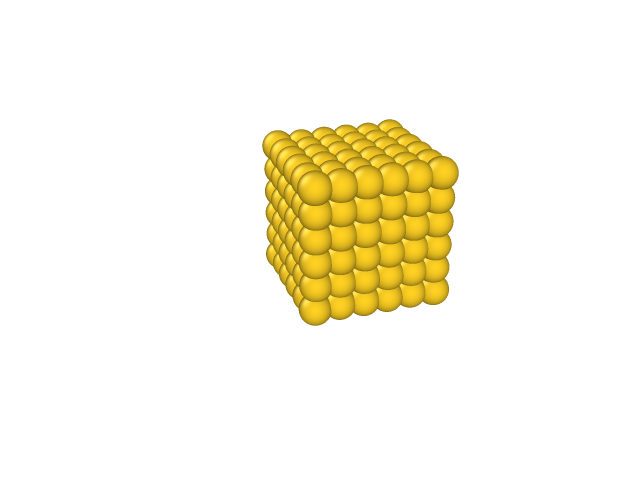
\includegraphics[trim={3.2cm 3.2cm 3.2cm 1.8cm},clip]{img/snap1.png}}
	\end{minipage}\hfill
	\begin{minipage}{.3\textwidth}
		\centering
		\resizebox{\columnwidth}{!}{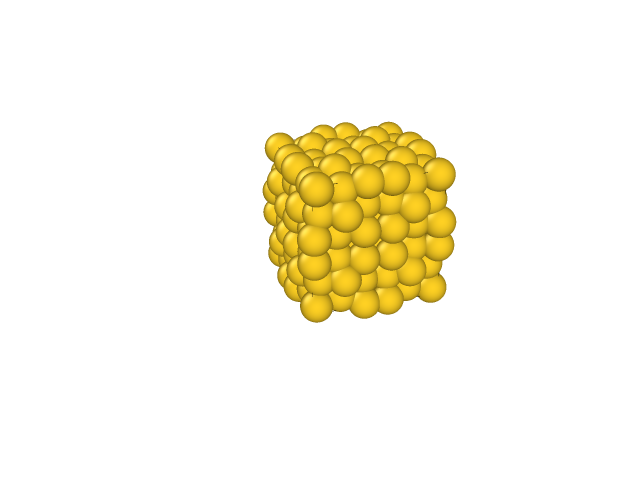
\includegraphics[trim={3.2cm 3.2cm 3.2cm 1.8cm},clip]{img/snap2.png}}
	\end{minipage}\hfill
	\begin{minipage}{.3\textwidth}
		\centering
		\resizebox{\columnwidth}{!}{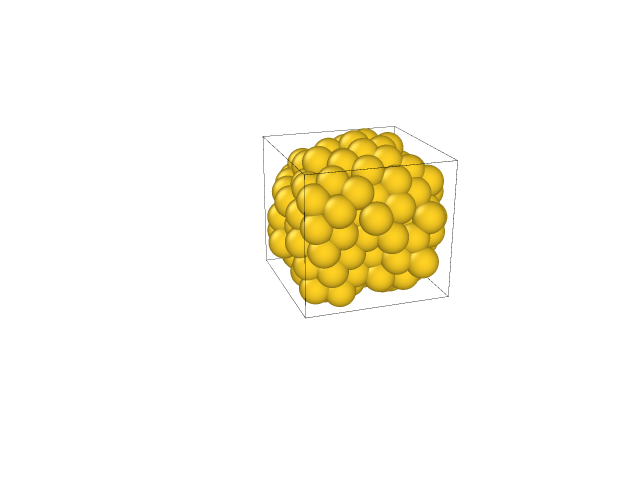
\includegraphics[trim={3.2cm 3.2cm 3.2cm 1.8cm},clip]{img/snap3.png}}
	\end{minipage}
	\caption{OVITO visualization of a cubic lattice with Berendsen thermostat.\\
		Initial configuration: cube with 6 atoms along each axis, distance between neighbors is $r=2^{1/6}\sigma$ -- the optimum point of Lennard Jones potential.\\	
		Time is in Lennard Jones potential units.\\
		Lennard Jones parameters are: $m=1$ LJ units of mass, $\sigma$ = 2Å, $\epsilon$=1eV.\\
		Total simulation time \( 100 \sqrt{m\sigma^2 / \epsilon} \), simulation state save interval \( 1 \sqrt{m\sigma^2 / \epsilon} \).
		Visualized at time points 0, 4, and 10 $\sqrt{m\sigma^2 / \epsilon}$.
	}
	\label{fig:first_simulation_ovito}
\end{figure*}

\clearpage

We connect a heat bath, also called a thermostat, to the atomic system to prevent boiling or evaporation. Following tasks should be solved:

\begin{itemize}
	\item Find an optimal timestep for the simulation without thermostat. We should take the largest possible value at which the total energy stays constant. Similar to the first simulation, I checked several timesteps and chose $\Delta t = 0.001 \sqrt{m\sigma^2 / \epsilon}$ that caused least total energy drift (Fig.~\ref{fig:total_energy_check}).
	\item Select a target temperature for the thermostat. I chose room temperature $T_0 = 300$ K.
	\item Find an optimal relaxation time for the thermostat. It should be much larger than the simulation timestep $\tau \gg \Delta t$, but low enough to reduce the temperature of the system. For the cubic lattice, I found that with $\tau = 1 \sqrt{m\sigma^2 / \epsilon}$ the target temperature is reached fast enough, and with higher values the target 300 K is reached too slowly.
	\item Use the two-stage equilibration strategy: set relaxation time firstly to a small value and increase it afterwards. To minimally disturb the system, we need to find the shortest equilibration time $\tau_{EQ}$. I found that with $\tau_{EQ} = 20 \sqrt{m\sigma^2 / \epsilon}$ the target temperature was reached. After that point I set relaxation time $\tau$ to the total duration of the simulation.
\end{itemize}

OVITO visualization of the system is shown in Fig.~\ref{fig:first_simulation_ovito}.

{\bf Thermostat implementation test.} Testing is very simple: because Berendsen thermostat modifies the speed of each atom separately, it's enough to test the method on just one atom. Let the initial position of the atom be $\mat{r}(1, 0, 0)$ and velocity $\mat{v}(1, 0, 0)$, Lennard Jones potential parameters $m=1$ LJ units of mass, $\sigma$=1Å, $\epsilon$=1eV, time step $\Delta t=1 \sqrt{m\sigma^2 / \epsilon}$.

First test: if relaxation time $\tau = \Delta t$, the desired temperature $T_0 = 0.5$ K must be reached in one step.

Second test: temperature should exponentially approach the desired value. If we set $\tau = 10 \Delta t$, after 50 steps the temperature should be within 0.01 from the desired value $T_0 = 1000$ K.


{\bf Implementation}
\begin{lstlisting}[breaklines]
src/lattice.cpp
src/lattice.h
src/thermostat.cpp
src/thermostat.h,
tests/test_thermostat.cpp
milestones/05/main.cpp
\end{lstlisting}

\clearpage

\subsection*{Neighbor list}

\begin{figure*}[htb]
	\centering
	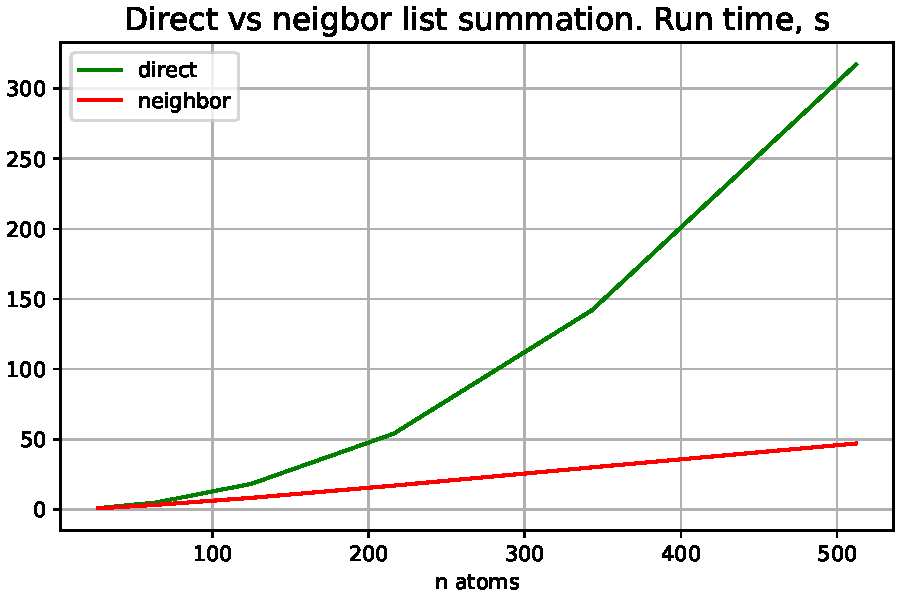
\includegraphics[width=.8\linewidth]{img/milestone06-time.pdf}
	\caption{Without neighbor list, time scales quadratically with number of atoms.\\
	Initial configuration: cube with $n$ atoms along each axis, distance between neighbors is $r=2^{1/6}\sigma$ -- the optimum point of Lennard Jones potential.\\	
	Lennard Jones parameters are $m=1$  LJ units of mass, $\sigma$ = 2Å, $\epsilon$=1 eV.\\
	Total simulation time \( 100 \sqrt{m\sigma^2 / \epsilon} \), simulation state save interval \( 1 \sqrt{m\sigma^2 / \epsilon} \).\\
	The provided implementation of neighbor lists is used. Cutoff radius is \( 3 \sigma \) to allow speedup, but not miss interactions. Tested on following cube sizes: $3^3=27, 4^3=64, 5^3=125, 6^3=216, 7^3=343, 8^3=512, 9^3=729$.
	}
	\label{fig:neighbor}
\end{figure*}

The neighbor list data structure speeds up nearby atom search for forces computation. Execution time on clusters of different sizes is compared in Fig.~\ref{fig:neighbor}

{\bf Implementation}
\begin{lstlisting}[breaklines]
src/neighbors.cpp, src/neighbors.h,
tests/test_neighbors.cpp,
src/lj.cpp, src/lj.h,
tests/test_thermostat.cpp
milestones/06/main.cpp
\end{lstlisting}

{\bf Run details}\\
Optimization level 3 must be enable before compilation.\\
Run: \verb|cd buildDir/milestones/06; time ./milestone06 [n]|\\
Plot with \verb|plot/time_lineplot.ipynb|

\subsection*{Heating experiment}

In this experiment we use the EAM potential with real physical units: $[l]$ = 1 Å, $[E]$ = 1 eV, $[t]$ = 1 fs, $[m]$ = 0,009649 g/mol. We want to estimate properties of several gold clusters when they melt, for that we need to heat them up, plot the total energy vs temperature and analyse the plot. I simulated the Makay-923 and Makay-3871 Makay clusters, introduced in \cite{MakayOriginal} and implemented by Dr Lars Pastewka in \cite{MakayPastewka}, and additionally generated Whisker-6950 using the \verb|make_whisker.py| script.

{\bf Finding an optimal timestep.} Firstly, we must find an optimal timestep that would minimize total energy drift. I took the Makay-923 cluster for testing, and like in previous experiments, I checked the total energy drift for several timesteps (Fig.~\ref{fig:total_energy_07}). With $\Delta t > 20$ fs the system exploded. As the cluster is quite big and slows down computation, it's better to pick a larger timestep $\Delta t = 10$ fs.

\begin{figure*}[htb]
	\centering
	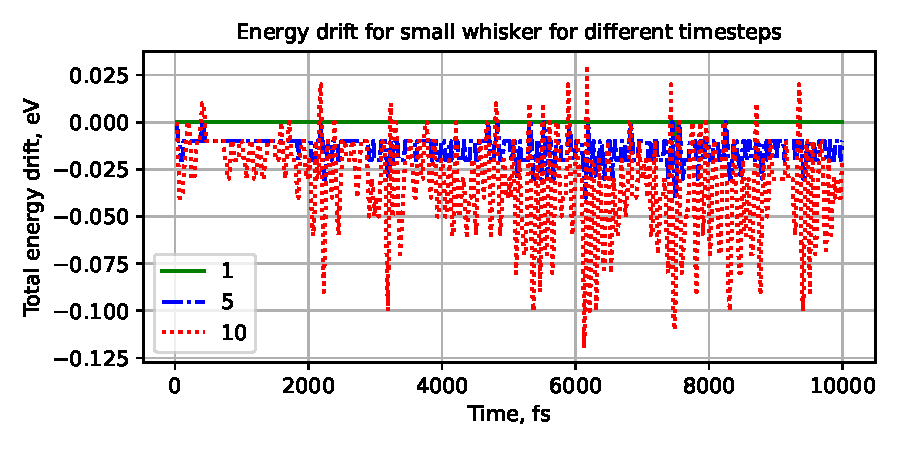
\includegraphics[width=.9\linewidth]{img/milestone07-energy.pdf}
	\caption{Choosing the optimal time step for the small whisker for Ducastelle EAM potential. All shown simulations drift less than 1 eV per 10 000 steps, so we can accept $\Delta t = 10$ fs.\\
		I plot the total energy minus its initial value.\\
		Timesteps in the legend are in fs.\\
		Initial configuration from file {\bf cluster\_923.xyz}.\\
		Total simulation time 10 ps, simulation state save interval 20 fs.
		No thermostat or heat addition is used.}
	\label{fig:total_energy_07}
\end{figure*}

\clearpage

\subsubsection*{Adding heat}

To add a fixed amount of energy $Q$ we scale the velocities by $\lambda$:

\[
\begin{aligned}
	E_k &= \frac{1}{2} \sum_i m v_i^2 \\
	E_k + Q &= \frac{1}{2} \sum_i m (\lambda v_i)^2 = \lambda^2 \frac{1}{2} \sum_i m v_i^2 \\
	E_k + Q &= \lambda^2 E_k \\
	\lambda^2 &= 1 + \frac{Q}{E_k} \\
\end{aligned}
\]

{\centering\framed{ \( \lambda = \sqrt{1 + \frac{Q}{E_k}} \) }\\}

Latent heat is the energy to transform from solid to liquid state. During melting the temperature stays the same, but potential energy increases. Heat capacity is the coefficient $dE/dT$ of linear relation between $E_{tot}$ and $T$.

In the experiment, we need to deposit such an amount of heat that it doesn't disturb the system too much, but reaches the melting point. I chose $\Delta Q$ as 20 eV, 100 eV, and 200 eV for small Mackay cluster, big Mackay cluster and the whisker respectively. I don't use Berendsen thermostat because it makes the experiment meaningless by arbitrarily adding or removing energy.

\subsubsection*{Computing melting point, heat capacity and latent heat}
I wrote a program to estimate the desired values from the energy-temperature plot.

\begin{itemize}
	\item Melting point: as the simulation doesn't have truly constant melting temperature, I take the middle point between the end of linear region for solid state and beginning of linear region for liquid state on the energy-temperature plot (Fig.~\ref{fig:heat-makay1},~\ref{fig:heat-makay2},~\ref{fig:heat-whisker}).
	\item To measure the heat capacity coefficient I take two far away points on the energy-temperature plot and compute $(E_2-E_1)/(T_2-T_1)$.
	\item To measure latent heat I extrapolate the lines for solid state and liquid state to the assumed melting point and take the difference in energies (Fig.~\ref{fig:heat-estimated}).
\end{itemize}

\begin{figure*}[h!]
	\centering
	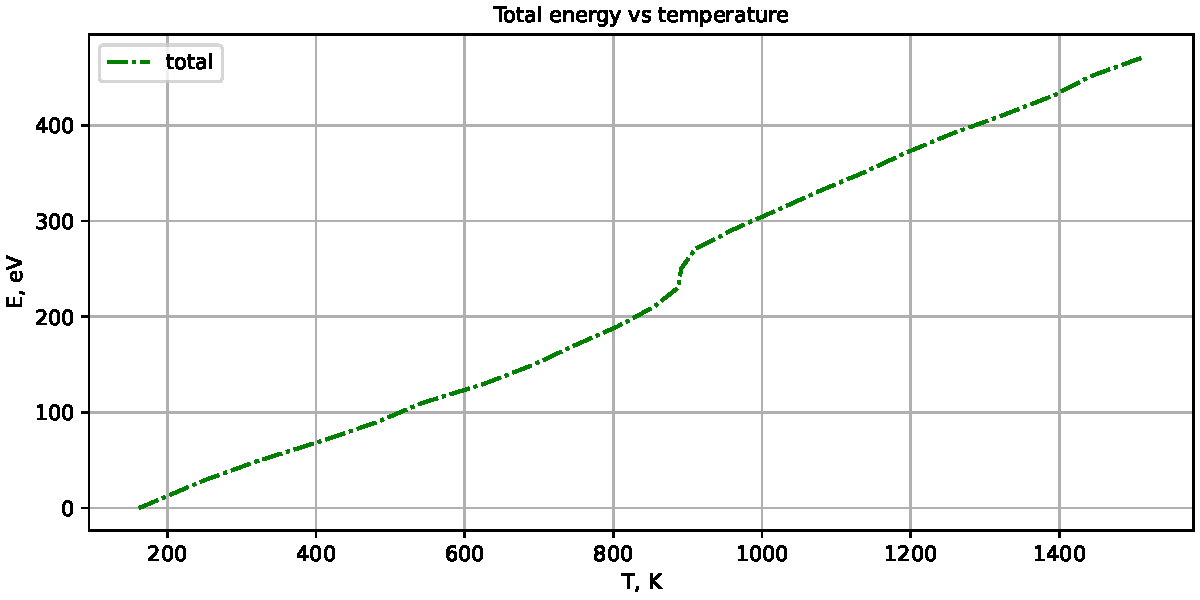
\includegraphics[width=.95\linewidth]{img/milestone07-small.pdf}
	\caption{Total energy (eV) vs temperature (K) for Makay-923.\\
	 	EAM potential cutoff at 9Å. Initial configuration from file {\bf cluster\_923.xyz}.\\
		$\Delta t = 10$ fs, total simulation time 100 000 fs, simulation state save interval 4000 fs, heat deposit interval 4000 fs.
		No thermostat is used.}
	\label{fig:heat-makay1}
\end{figure*}

\begin{figure*}[h!]
	\centering
	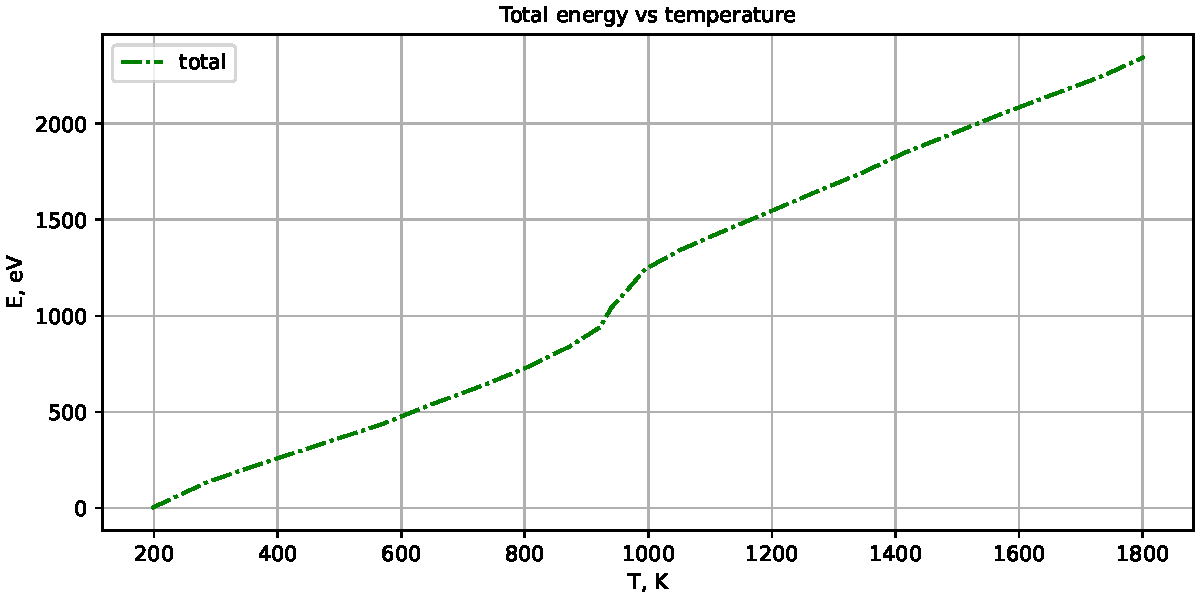
\includegraphics[width=.95\linewidth]{img/milestone07-large.pdf}
	\caption{Total energy (eV) vs temperature (K) for Makay-3871.\\
	EAM potential cutoff at 9Å. Initial configuration from file {\bf cluster\_3871.xyz}.\\
	$\Delta t = 10$ fs, total simulation time 100 000 fs, simulation state save interval 4000 fs, heat deposit interval 4000 fs.
	No thermostat is used.}
	\label{fig:heat-makay2}
\end{figure*}

\clearpage

\begin{figure*}[h!]
	\centering
	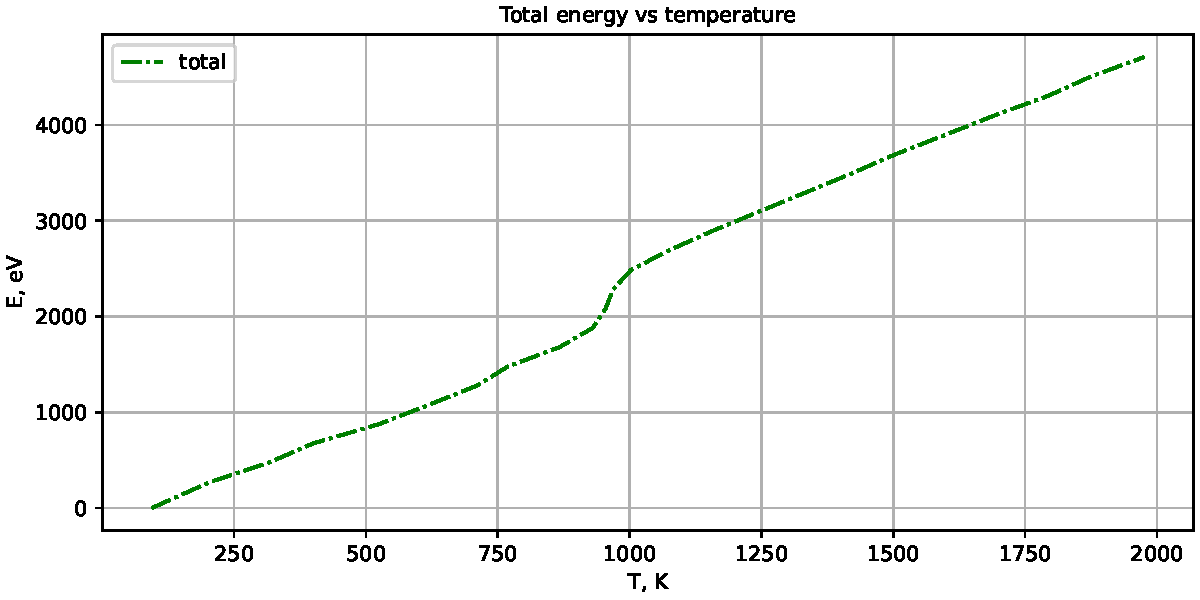
\includegraphics[width=.95\linewidth]{img/milestone07-whisker.pdf}
	\caption{Total energy (eV) vs temperature (K) for Whisker-6950.\\
	EAM potential cutoff at 9Å. Initial configuration from the generated whisker (see run details).\\
	$\Delta t = 10$ fs, total simulation time 100 000 fs, simulation state save interval 4000 fs, heat deposit interval 4000 fs.
	No thermostat is used.}
	\label{fig:heat-whisker}
\end{figure*}

\begin{figure*}[h!]
	\centering
	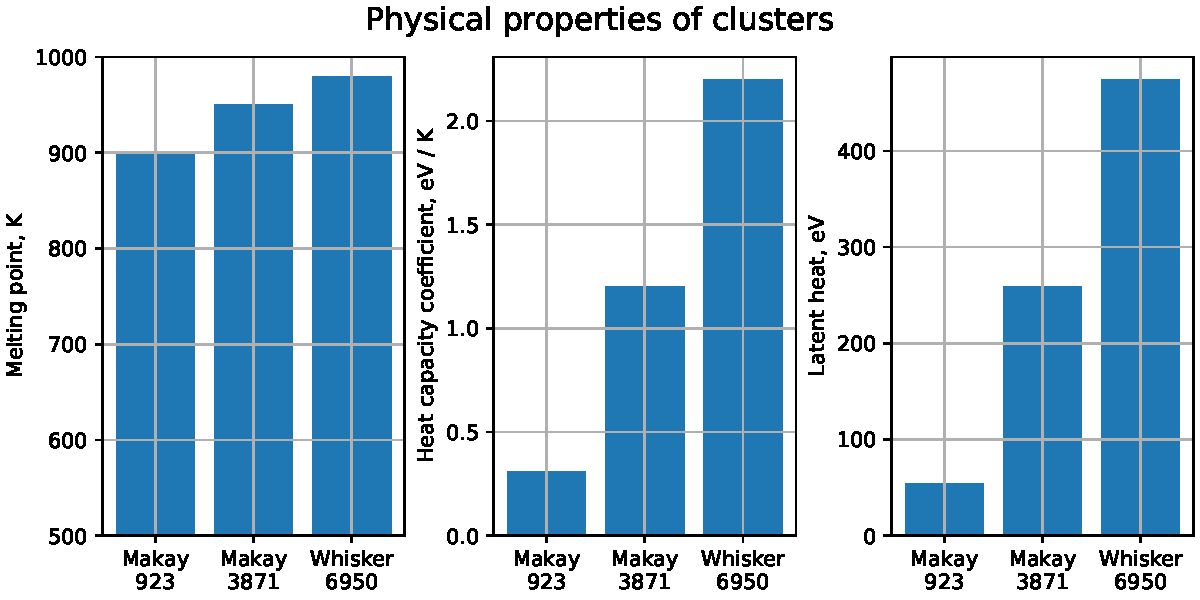
\includegraphics[width=.9\linewidth]{img/milestone07-bar.pdf}
	\caption{Estimated Melting point (K), Heat capacity coefficient (eV / K), Latent heat (eV) for each cluster.\\
	EAM potential cutoff at 9Å. Initial configuration from corresponding file.\\
	$\Delta t = 10$ fs, total simulation time 100 000 fs, simulation state save interval 4000 fs, heat deposit interval 4000 fs.
	No thermostat is used.}
	\label{fig:heat-estimated}
\end{figure*}

\newpage

{\bf Implementation}
\begin{lstlisting}[breaklines]
src/ducastelle.h,
src/ducastelle.cpp,
milestones/07/main.cpp
\end{lstlisting}

{\bf Run details}
\begin{itemize}
	\item Generate Whisker-6950: \verb|python make_whisker.py| with parameters \verb|radius = 15; size = [14, 10, 50]|
	\item Run: \verb|cd buildDir/milestones/07|
	\item Logs are saved in \verb|buildDir/milestones/07|
	\item Plot with \verb|plot/milestone07.ipynb|
	
\end{itemize}

\newpage

\subsection*{Parallelization}

In this experiment we distribute the atomic system across multiple processes for parallelization. We define the domain -- the coordinate limits for each dimension: $\Omega = [0, L_x] \times [0, L_y] \times [0, L_z]$ and divide each dimension into $N_x, N_y, N_z$ equal parts respectively. I tested the approach on the gold cluster Mackay-3871 and verified correctness of implementation by running simulation on 1, 4, 8 processes. I monitored the total energy and temperature, which are the same across all runs, thus the implementation is correct (Fig.~\ref{fig:parallel-1},~\ref{fig:parallel-2},~\ref{fig:parallel-3}).

\subsubsection*{Choice of domain size and grid}

The domain must include all the atoms in our system. We can see in OVITO visualization of the cluster that [0, 50Å] $\times$ [0, 50Å] $\times$ [0, 50Å] is a large enough domain. The grid size $(N_x, N_y, N_z)$ can be chosen arbitrarily, thus I chose $(1, 1, 1)$, $(1, 2, 2)$, and $(2, 2, 2)$.

\subsubsection*{Disappearing atoms problem}

If the domain is not periodical, atoms that are close to the boundary may disappear from simulation and cause explosion -- we need to add a margin at the beginning and end of the domain to prevent this. I translated each atom $\mat{r_i}(x, y, z)$ to  $\mat{r_i}(x + 5, y + 5, z + 5)$ (lengths in Å) and increased the domain size $L = L_x = L_y = L_z = 60$ Å, meaning we have at least 5Å margin at both ends of the domain for each dimension.

\subsubsection*{Simulation parameters}

No thermostat is needed for these experiments, as the icosahedron cluster is very stable. I take the simulation timestep $\Delta t = 10$ fs from the previous experiment. 



\subsubsection*{Run details}
\begin{itemize}
	\item Input total number of processes, domain size and grid size as command arguments:\\
	\verb|mpirun -n n_processes --oversubscribe ./milestone08 lx ly lz nx ny nz|
	\item Outputs are generated in \verb|buildDir/milestones/08|
	\item Plot with \verb|plot/milestone08.ipynb|
\end{itemize}

\begin{figure*}[h!]
	\centering
	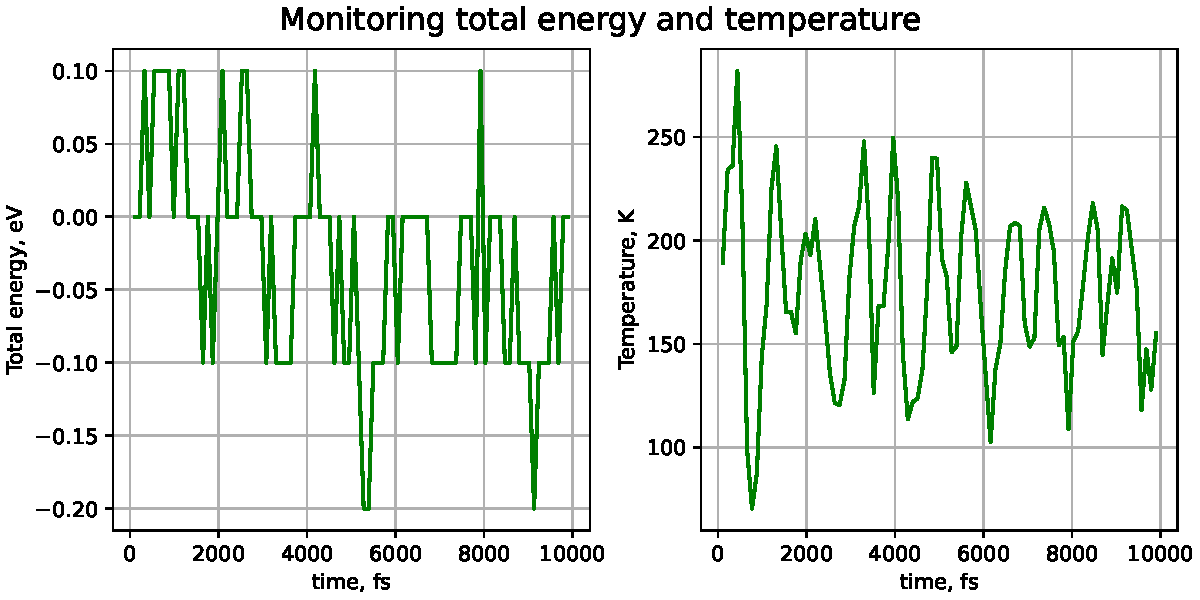
\includegraphics[width=.8\linewidth]{img/milestone08-1proc.pdf}
	\caption{Parallelized with 1 process.\\
	Domain size [0, 60Å] $\times$ [0, 60Å] $\times$ [0, 60Å], grid size (1, 1, 1).\\
	EAM potential cutoff 9Å, ghost atom cutoff 18Å. Initial configuration from file {\bf cluster\_3871.xyz}.\\
	$\Delta t = 10$ fs, total simulation time 10 000 fs, simulation state save interval 100 fs. No thermostat is used.}
	\label{fig:parallel-1}
\end{figure*}

\begin{figure*}[h!]
	\centering
	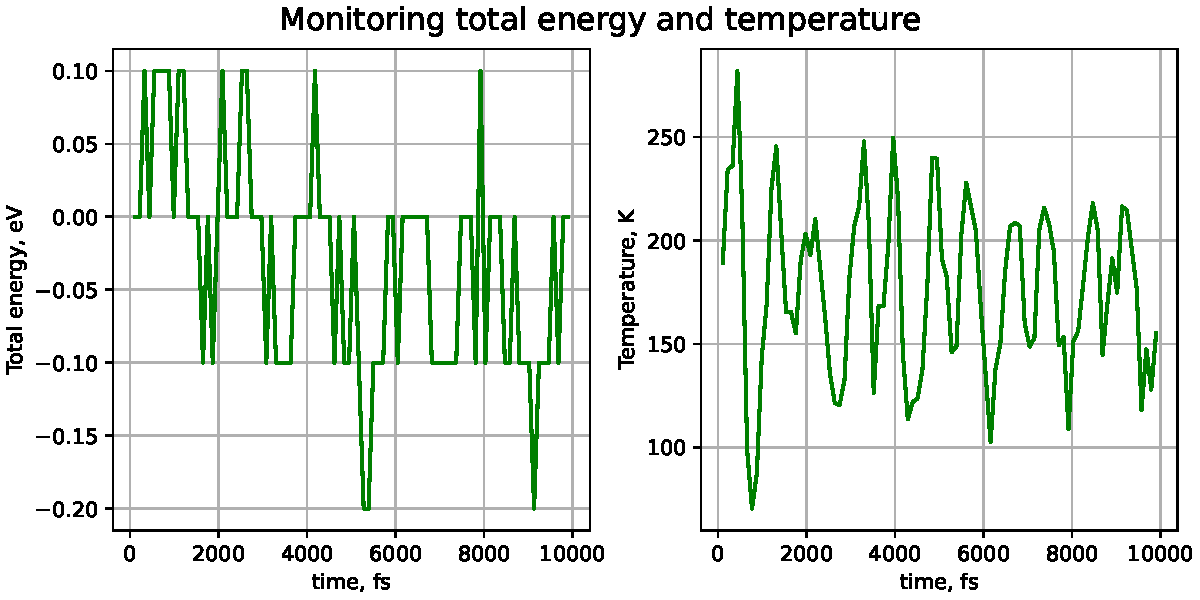
\includegraphics[width=.85\linewidth]{img/milestone08-4proc.pdf}
	\caption{Parallelized with 4 processes.\\
	Domain size [0, 60Å] $\times$ [0, 60Å] $\times$ [0, 60Å], grid size (1, 2, 2).\\
	EAM potential cutoff 9Å, ghost atom cutoff 18Å. Initial configuration from file {\bf cluster\_3871.xyz}.\\
	$\Delta t = 10$ fs, total simulation time 10 000 fs, simulation state save interval 100 fs. No thermostat is used.}
	\label{fig:parallel-2}
\end{figure*}

\clearpage

\begin{figure*}[h!]
	\centering
	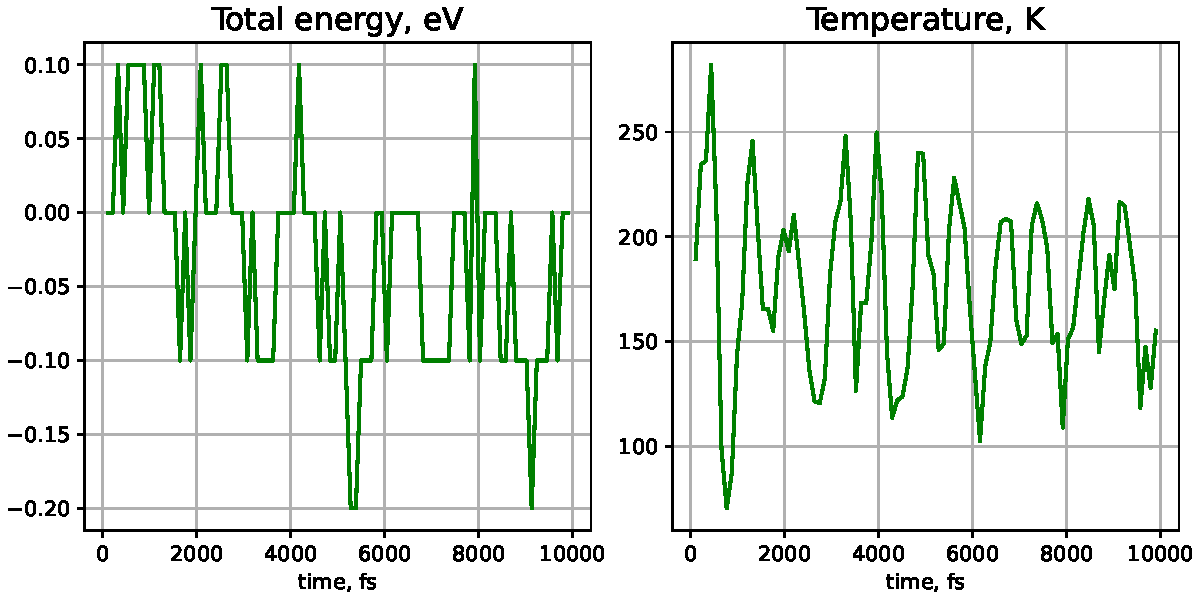
\includegraphics[width=.85\linewidth]{img/milestone08-8proc.pdf}
	\caption{Parallelized with 8 processes.\\
	Domain size [0, 60Å] $\times$ [0, 60Å] $\times$ [0, 60Å], grid size (2, 2, 2).\\
	EAM potential cutoff 9Å, ghost atom cutoff 18Å. Initial configuration from file {\bf cluster\_3871.xyz}.\\
	$\Delta t = 10$ fs, total simulation time 10 000 fs, simulation state save interval 100 fs. No thermostat is used.}
	\label{fig:parallel-3}
\end{figure*}


\subsubsection*{Implementation}
\begin{lstlisting}[breaklines]
src/mpi_support.h
src/domain.h
src/domain.cpp
milestones/08/main.cpp
\end{lstlisting}

\clearpage % works for figures too!

\subsection*{Pulling a gold nanowire}

In the final experiment we stretch a golden whisker by using a periodical domain along Z axis (Fig.~\ref{fig:whisker-small-defect}). Our objective is to analyze the stress tensor (similar to pressure) depending on the elongation of the whisker under different temperatures, strain rates, and whisker sizes.

\subsubsection*{Domain size and grid}

I implemented automatic domain size computation so that I don't have to input it manually. The $L_x$ and $L_y$ domain size can be chosen freely, given a sufficient offset from the domain edge. The whisker files already have at least 5Å offset so it's reasonable to take $[0, max(\mat{r}_i(x)) + 5\text{Å}]$ as domain size for X dimension and similarly for Y dimension. The computed domain sizes for the whiskers are:

\begin{itemize}
	\item \verb|whisker_small.xyz|: $L_x$ = 37Å, $L_y$ = 34Å
	\item \verb|whisker_large.xyz|: $L_x$ = 80Å, $L_y$ = 74Å
\end{itemize}

The $L_z$ is much harder to set correctly, because the domain is periodical across Z axis, and should simulate an infinitely long whisker. The distance between the end and the periodical beginning of the whisker must be close to the optimum of EAM potential, otherwise the system will explode or disconnect. I tried out different distances, and the domain size $[0, max(\mat{r}_i(z)) + 1\text{Å}]$ worked the best. The following domain size was estimated:

\begin{itemize}
	\item \verb|whisker_small.xyz|: $L_z$ = 144.5Å
	\item \verb|whisker_large.xyz|: $L_z$ = 288.8Å
\end{itemize}

Domain decomposition is done automatically across Z axis only. Given N processes, the grid size $(N_x, N_y, N_z) = (1, 1, N)$.

\subsubsection*{Stress calculation}

Stress is the tension of the material under external force. It's similar to pressure, measured in Pascal $[f]/[l]^2 = [m]/([t]^2[l])$, the exact unit can be derived for EAM potential but it wasn't required for the report.

\[
\sigma =
\begin{pmatrix}
	\sigma_{xx} &\sigma_{xy} &\sigma_{xz}\\
	\sigma_{yx} &\sigma_{yy} &\sigma_{yz}\\
	\sigma_{zx} &\sigma_{zy} &\sigma_{zz}\\
\end{pmatrix}
\]

\[
\sigma = \cfrac{1}{V} \sum_{i<j} \mat{r}_{ij} \times \mat{f}^T_{ij} = \cfrac{1}{V} \sum_i^{N} \sum_{j=i}^{N+N_G} \mat{r}_{ij} \times \mat{f}^T_{ij},
\]

where $V$ is body volume, $\mat{r}_{ij}$ is position, $\mat{f}_{ij}$ is force, $N_G$ is the number of ghost atoms.

By stretching the whisker we are applying a force along Z axis to the plane that is perpendicular to the Z axis, so we are interested only in $\sigma_{zz}$. In simulation other components were close to 0. I computed the stress tensor by summing up the expression in each subdomain and then summing over the subdomains. I used a big averaging window because stress fluctuates a lot.

\subsubsection*{Thermostat strategy}
Temperature is kept constant using Berendsen thermostat. Like in the thermostat experiment, I set a low relaxation time for a short period to quickly reach the desired temperature and then increase the relaxation time. For all launches I set:

\begin{itemize}
	\item Equilibration time $\tau_{EQ}$ = 2000 fs
	\item Relaxation time during equilibration: $\tau_1$ = 500 fs
	\item Relaxation time after equilibration: $\tau_2$ = 5000 fs
\end{itemize}

\subsubsection*{Varying temperature and strain}

At room temperature the whisker breaks reasonably fast, so I chose several temperatures close to 300 K, several strain values and computed the stress vs time plot for pairwise combinations of temperature and strain.

\begin{itemize}
	\item Small whisker: $T$ = 300K, 350K, 400K; total strain is 10Å, 15Å
	\item Large whisker: $T$ = 300K, 350K; total strain is 20Å, 30Å
\end{itemize}

\subsubsection*{Visualizing defects}

For visualization of defects in OVITO I used Common Neighbor Analysis and added the slice operation to see the center of the whisker (Fig.~\ref{fig:whisker-small-defect}, Fig.~\ref{fig:whisker-large-defect}). To apply these modifications in OVITO GUI one must select ``Add Modification - Structure identification - common neighbor analysis'', and ``Add Modification - Modification - slice''.


\subsubsection*{Discussion}

We observe the stress over time. The stress tensor was averaged over 500 fs which allows us to see clear patterns of defect formation.

For the small whisker (Fig.~\ref{fig:whisker-small}), faster starin breaks the wire more significantly, because stress drops earlier and lower. At higher temperature of 350 K, compared to 300 K, metal is more elastic, it deforms earlier but stress recovers quicker. The plot with same strain and different temperatures shows again that with higher temperature the metal is more elastic.

Similar can be said about the large whisker (Fig.~\ref{fig:whisker-large}), although it oscillates a lot at first. We can see more gradual stress relief for hotter metal.


\begin{figure*}[h!]
	\centering
	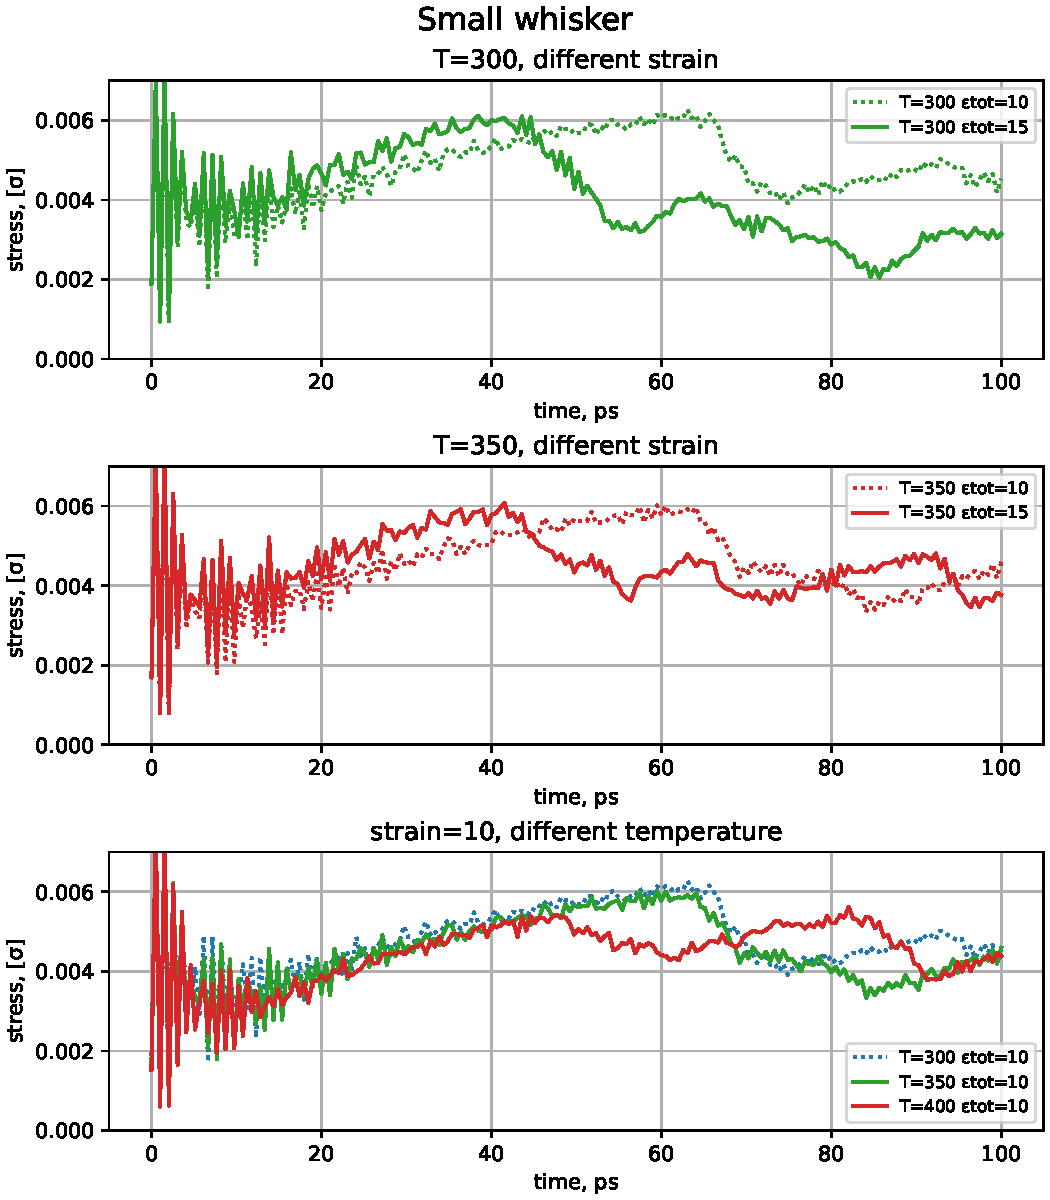
\includegraphics[width=.95\linewidth]{img/milestone09-small.pdf}
	\caption{Simulation with small whisker. Temperature $[t]=K$, total strain $[\epsilon]$ = Å, stress $\sigma$ is in pressure units in the EAM unit system.\\
	Initial domain size [0, 37Å] $\times$ [0, 34Å] $\times$ [0, 144.5Å], grid size (1, 1, 8).\\
	EAM potential cutoff 9Å, ghost atom cutoff 18Å. Initial configuration from file {\bf whisker\_small.xyz}.\\
	$\Delta t = 10$ fs, total simulation time 100 000 fs, simulation state save interval 500 fs, stress averaging interval is 500 fs.\\
	Berendsen thermostat $\tau_{EQ}$ = 2000 fs, $\tau_1$ = 500 fs, $\tau_2$ = 5000 fs (see text).
	}
	\label{fig:whisker-small}
\end{figure*}

\begin{figure*}[h!]
	\centering
	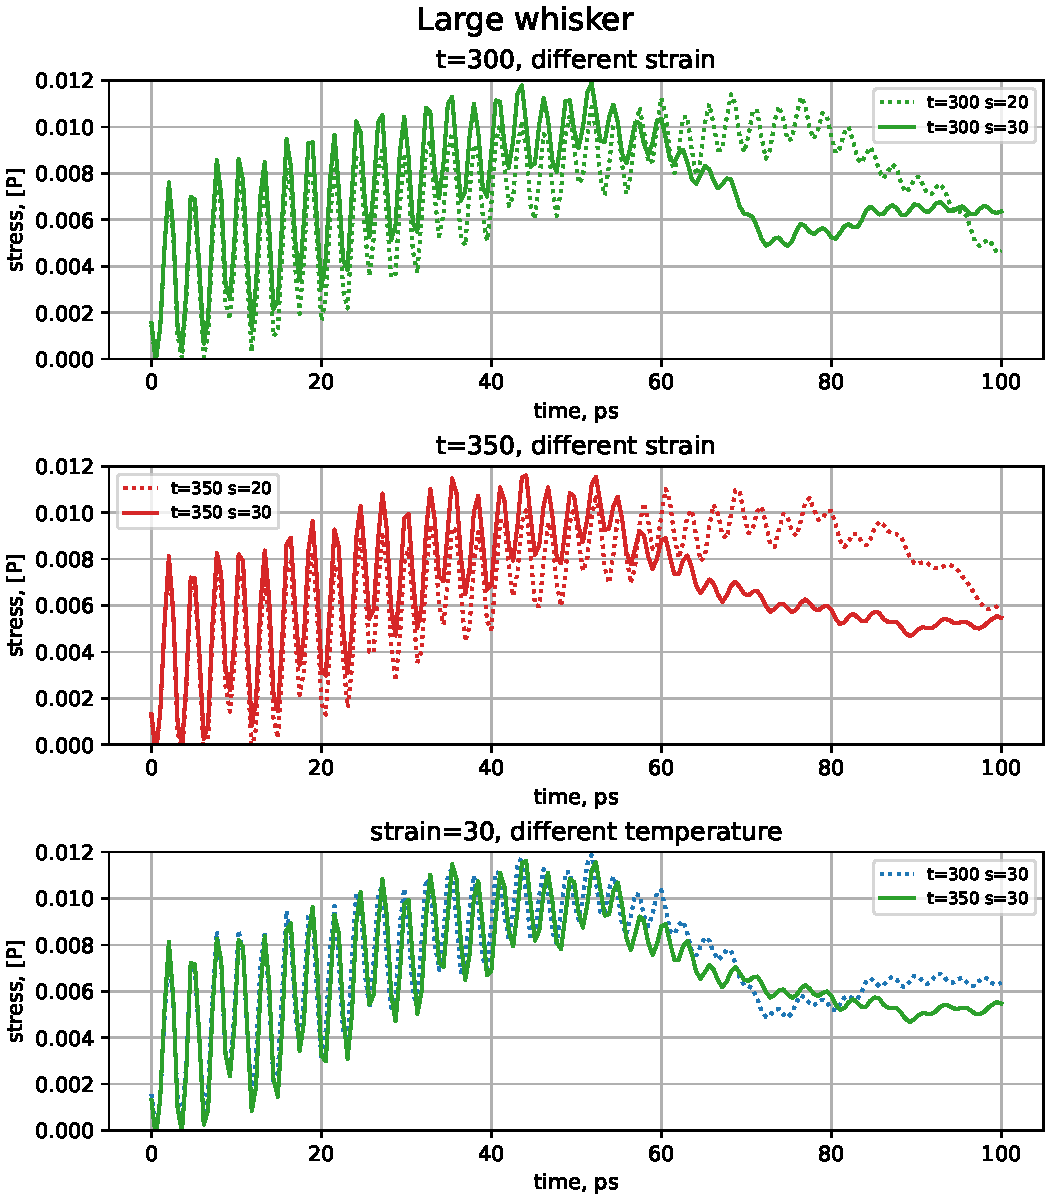
\includegraphics[width=.95\linewidth]{img/milestone09-large.pdf}
	\caption{Simulation with large whisker. Temperature $[t]=K$, total strain $[\epsilon]$ = Å, stress $\sigma$ is in pressure units in the EAM unit system.\\
		Initial domain size [0, 80Å] $\times$ [0, 74Å] $\times$ [0, 288.78Å], grid size (1, 1, 80).\\
		EAM potential cutoff 9Å, ghost atom cutoff 18Å. Initial configuration from file {\bf whisker\_large.xyz}.\\
		$\Delta t = 10$ fs, total simulation time 100 000 fs, simulation state save interval 500 fs, stress averaging interval is 500 fs.\\
		Berendsen thermostat $\tau_{EQ}$ = 2000 fs, $\tau_1$ = 500 fs, $\tau_2$ = 5000 fs (see text).
	}
	\label{fig:whisker-large}
\end{figure*}

\begin{figure*}[h!]
	\centering
	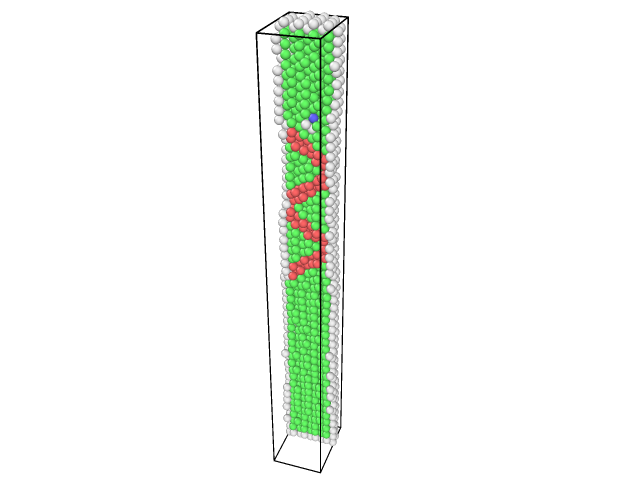
\includegraphics[width=.85\linewidth]{img/milestone09-small-300-10-pic.png}
	\caption{OVITO visualization of small whisker, 300 K, $\epsilon$ = 10Å,  image at 80 ps. The whisker is sliced in half, in red we see the break points.\\
	Temperature $[t]=K$, total strain $[\epsilon]$ = Å, stress $\sigma$ is in pressure units in the EAM unit system.\\
	Initial domain size [0, 37Å] $\times$ [0, 34Å] $\times$ [0, 144.5Å], grid size (1, 1, 8).\\
	EAM potential cutoff 9Å, ghost atom cutoff 18Å. Initial configuration from file {\bf whisker\_small.xyz}.\\
	$\Delta t = 10$ fs, total simulation time 100 000 fs, simulation state save interval 500 fs, stress averaging interval is 500 fs.\\
	Berendsen thermostat $\tau_{EQ}$ = 2000 fs, $\tau_1$ = 500 fs, $\tau_2$ = 5000 fs (see text).
	}
	\label{fig:whisker-small-defect}
\end{figure*}

\clearpage
\begin{figure*}[h!]
	\centering
	\begin{minipage}{.3\textwidth}
		\centering
		% w h w h_clip
		\resizebox{\columnwidth}{!}{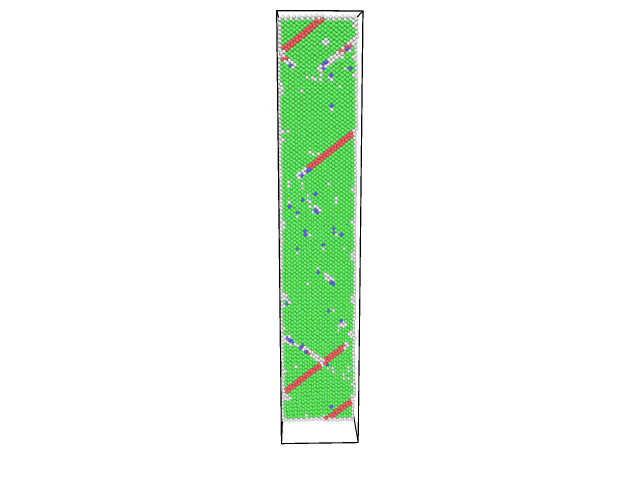
\includegraphics[trim={4.2cm 1.2cm 7.2cm 0.2cm},clip]{img/large-t350-s30-110.png}}
	\end{minipage}\hfill
	\begin{minipage}{.3\textwidth}
		\centering
		% w h w h_clip
		\resizebox{\columnwidth}{!}{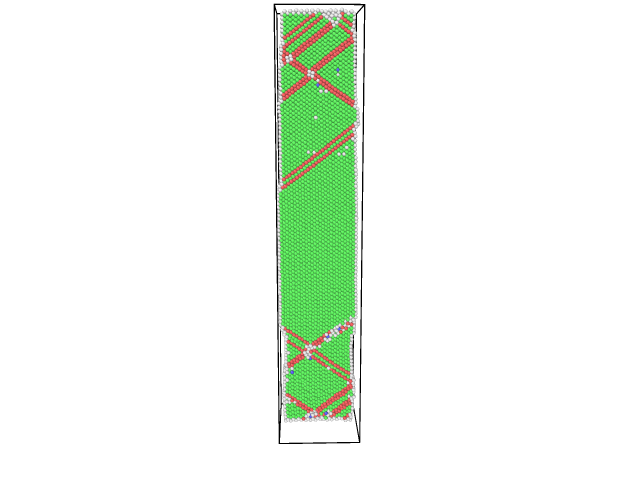
\includegraphics[trim={4.2cm 1.2cm 7.2cm 0.2cm},clip]{img/large-t350-s30-135.png}}
	\end{minipage}\hfill
	\begin{minipage}{.3\textwidth}
		\centering
		% w h w h_clip
		\resizebox{\columnwidth}{!}{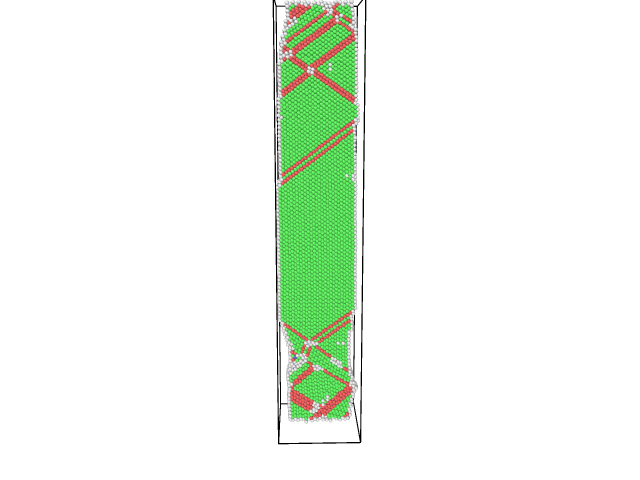
\includegraphics[trim={4.2cm 1.2cm 7.2cm 0.2cm},clip]{img/large-t350-s30-170.png}}
	\end{minipage}
	\caption{OVITO visualization of large whisker, 350 K, $\epsilon$ = 30Å Images at 60, 70, 80 ps. Temperature $[t]=K$, total strain $[\epsilon]$ = Å, stress $\sigma$ is in pressure units in the EAM unit system.\\
		Initial domain size [0, 80Å] $\times$ [0, 74Å] $\times$ [0, 288.78Å], grid size (1, 1, 80).\\
		EAM potential cutoff 9Å, ghost atom cutoff 18Å. Initial configuration from file {\bf whisker\_large.xyz}.\\
		$\Delta t = 10$ fs, total simulation time 100 000 fs, simulation state save interval 500 fs, stress averaging interval is 500 fs.\\
		Berendsen thermostat $\tau_{EQ}$ = 2000 fs, $\tau_1$ = 500 fs, $\tau_2$ = 5000 fs (see text).
	}
	\label{fig:whisker-large-defect}
\end{figure*}

\clearpage

{\bf Run details}
\begin{lstlisting}[breaklines]
cd buildDir/milestones/09
mpirun -n 4 --oversubscribe ./milestone09 300.0 10 whisker_small.xyz 1
sbatch run.job ./buildDir/milestones/09/milestone09 300.0 10.0 whisker_small.xyz 1
\end{lstlisting}

{\bf Implementation}
\begin{lstlisting}[breaklines]
milestones/09/main.cpp
\end{lstlisting}

\clearpage
\section{Conclusion}
\label{conclusion}

In this report I implemented a program that is capable of running a Molecular Dynamics simulation in parallel on a cluster. The report covers efficient implementation of the simulation using neighbor lists for the interatomic potentials, parallelization for multiple CPUs. The characteristics of materials were measured: energy of system, melting point, latent heat, heat capacity, stress force.

\newpage
{\small
	\bibliographystyle{plain}
	\bibliography{egbib}
}

\end{document}
